\section{Steel column-flat slab systems}\label{cft}
Concrete filled steel tube (CFT) columns have become more prevalent in construction practice during the last couple of decades providing relatively higher strength and ductility\citep{MORINO1998336}, reduced labor costs, less formwork, lower reinforcement requirements and ease of concrete pour compared to conventional reinforced concrete columns \citep{yan2011,wang2014}. 


\begin{figure}\centering
    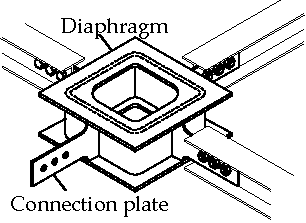
\includegraphics[width=\columnwidth]{Figures/s2004f3.pdf}
    \caption{CFT column-flat plate connection studied by \cite{satoh2004experimental,yamaguchi2008experimental}.}
    \label{s2004f3}
    \end{figure}
\begin{figure}\centering
    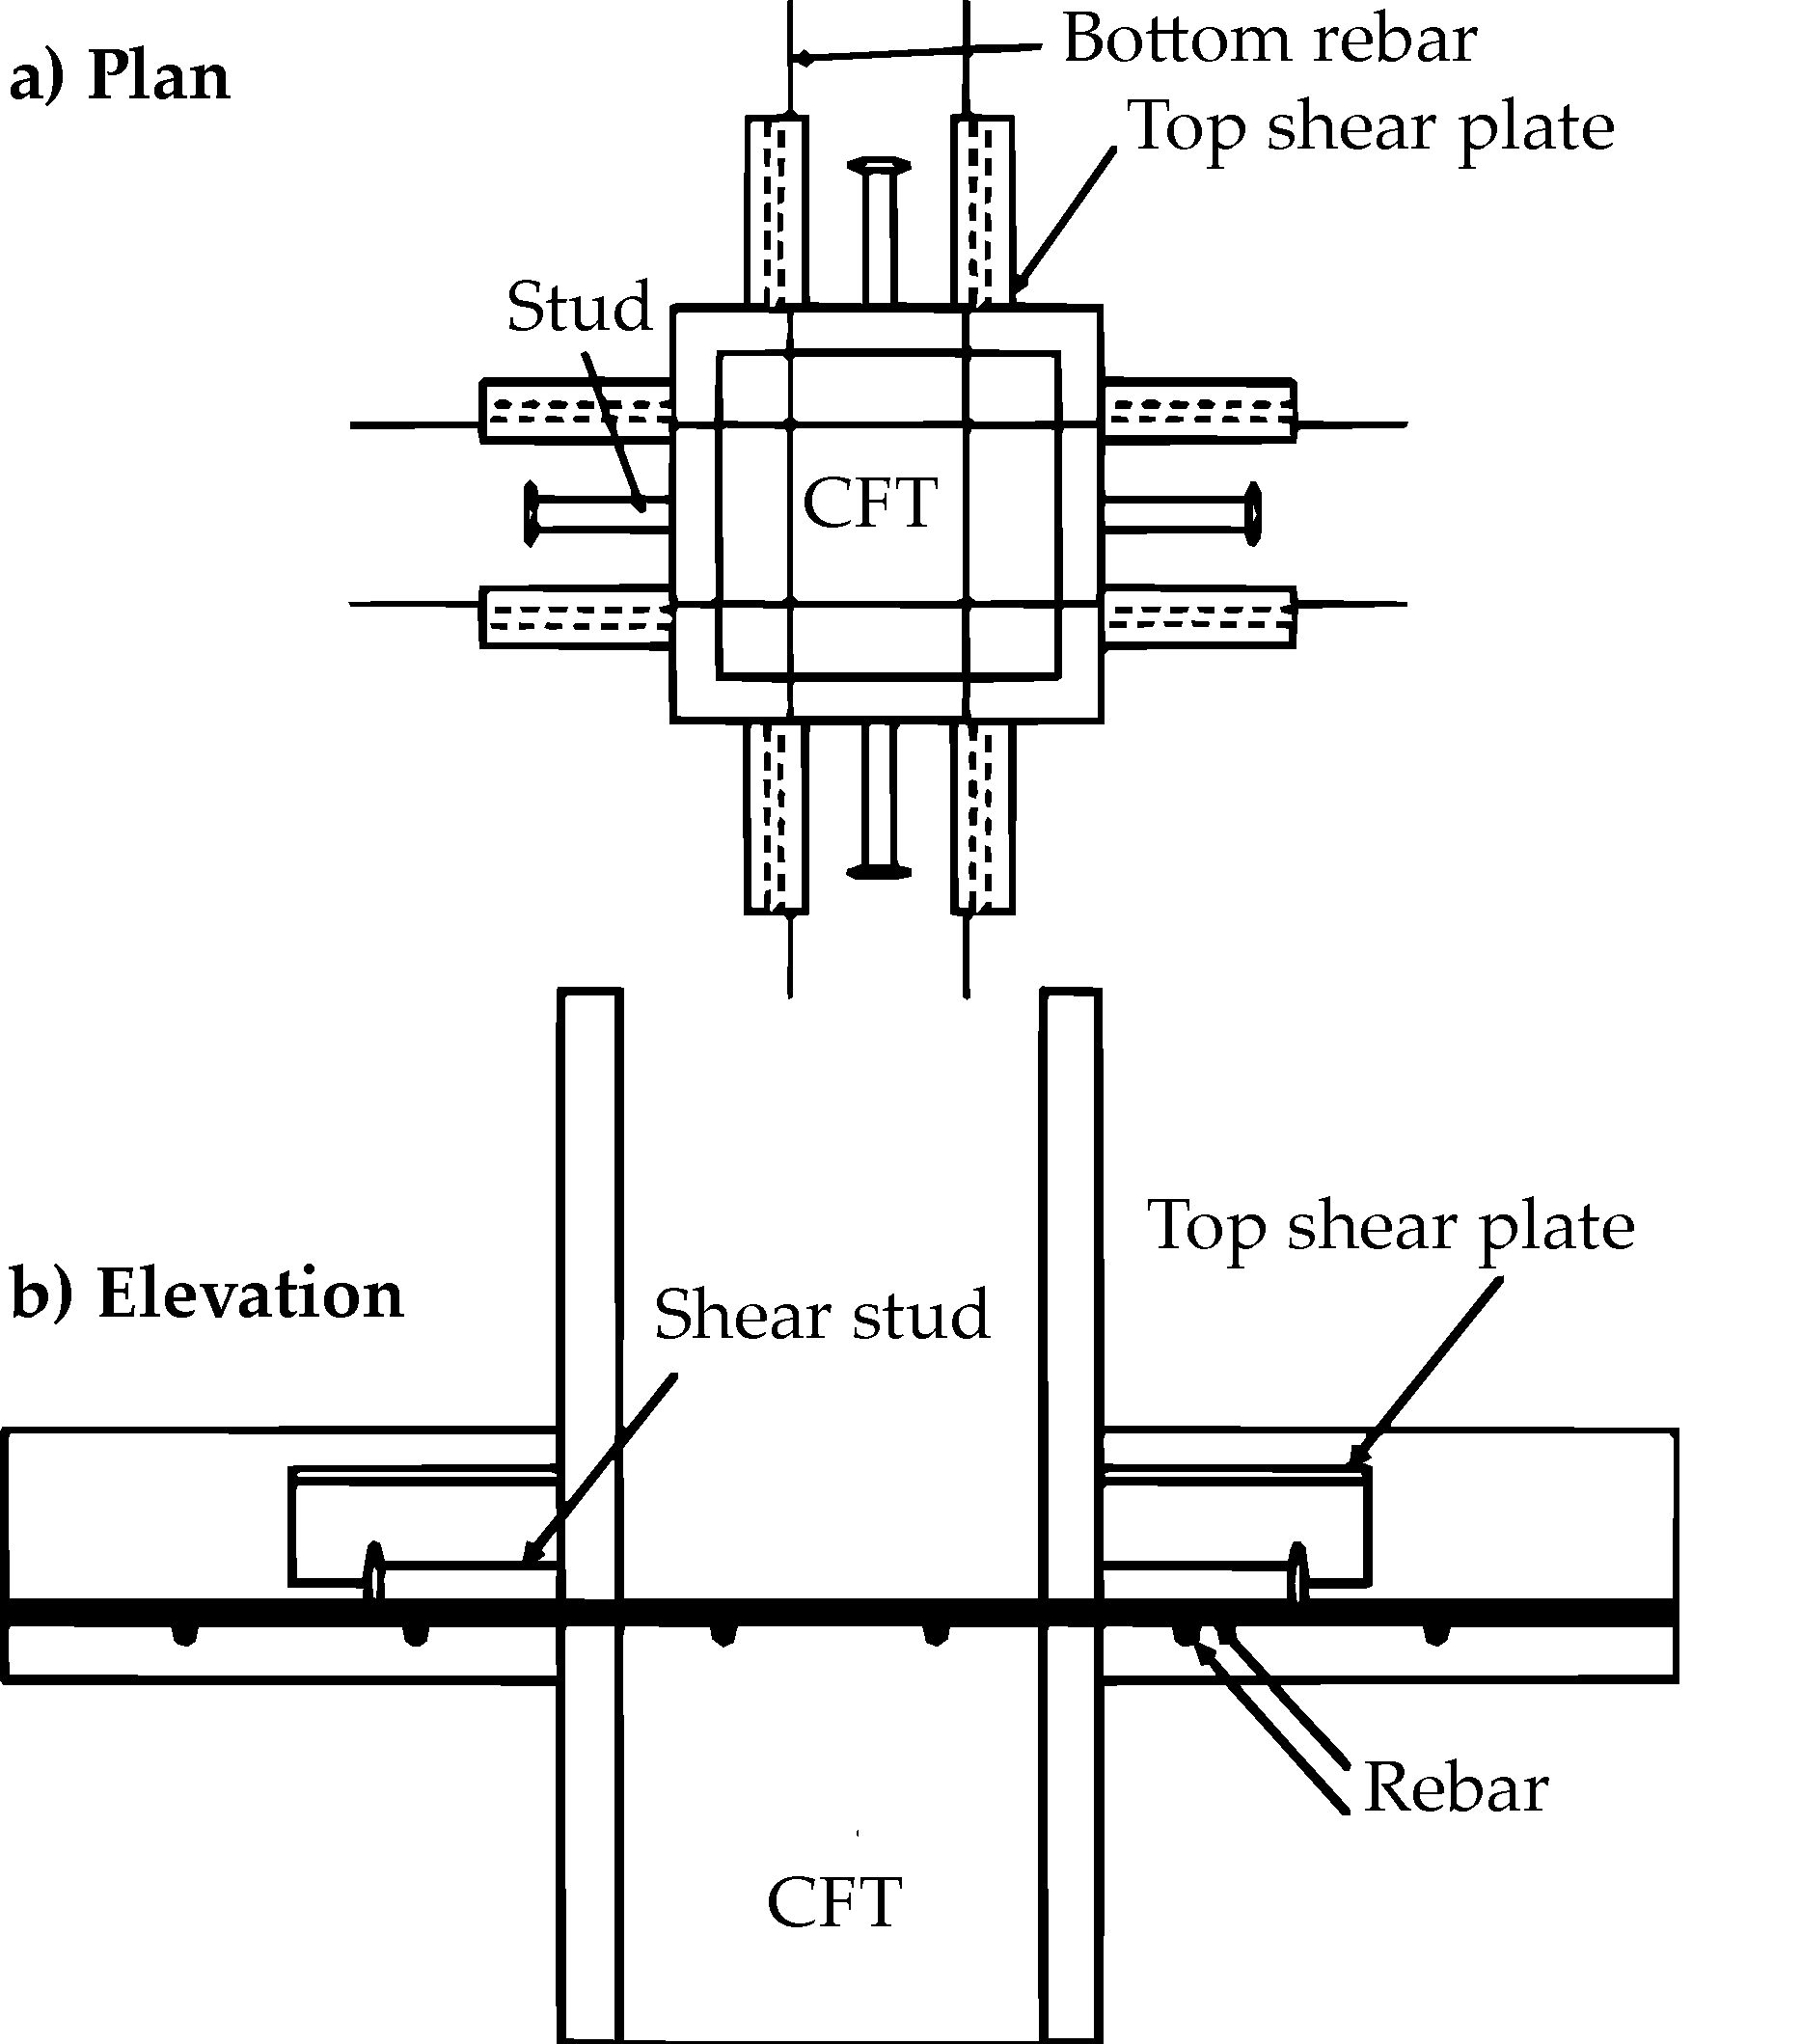
\includegraphics[width=\columnwidth]{Figures/l2005.pdf}
    \caption{CFT column-flat plate connection proposed by \cite{lee2005}.}
    \label{l2005}
    \end{figure}
\begin{figure}\centering
    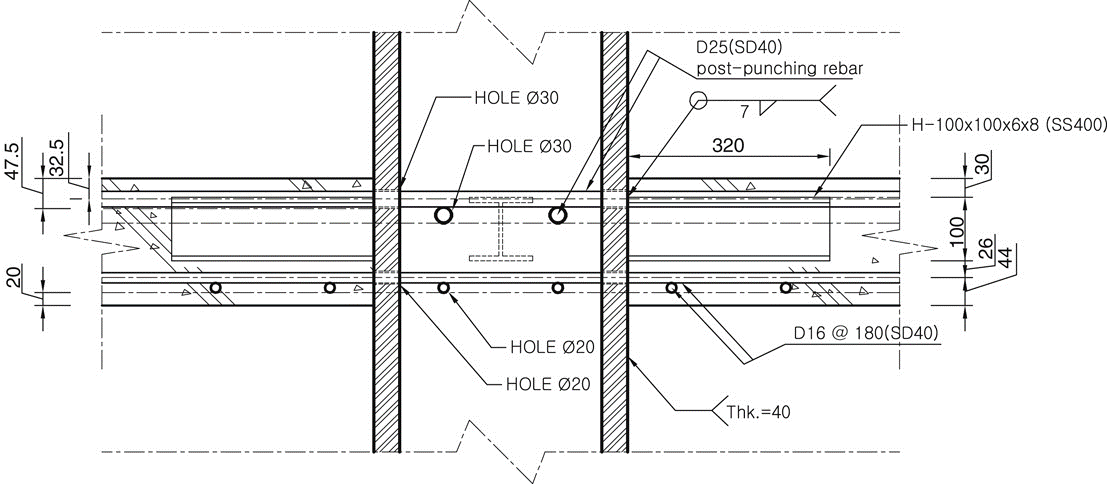
\includegraphics[width=\columnwidth]{Figures/l2008f2b.png}
    \caption{FPP-SH CFT column-flat plate connection specimen\citep{LEE2008418}.}
    \label{l2008f2b}
    \end{figure}
    
    \begin{figure}\centering
    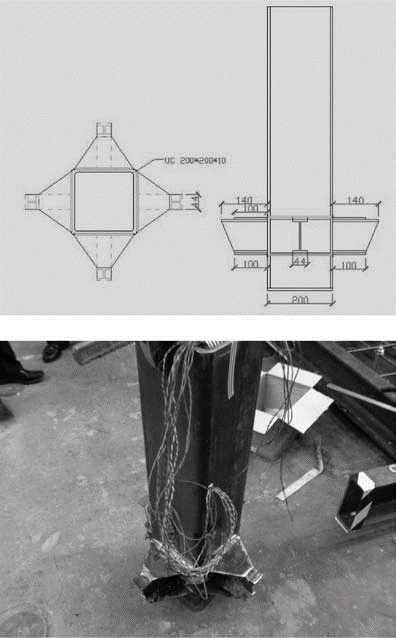
\includegraphics[width=\columnwidth]{Figures/y2009f3.png}
    \caption{\cite{yan2008} shearhead specimen.}
    \label{y2009f3}
    \end{figure}
\begin{figure}\centering
    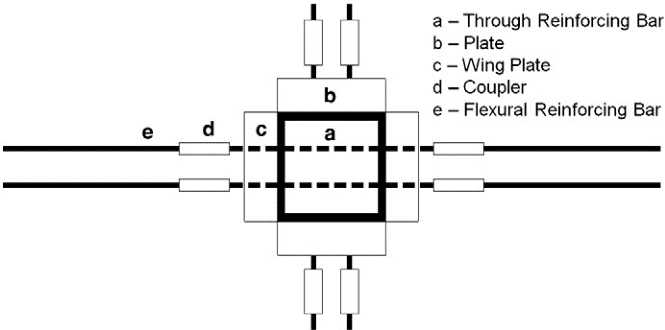
\includegraphics[width=\columnwidth]{Figures/j2013f9.png}
    \caption{Detail proposed by \cite{JU2013297}.}
    \label{j2013f9}
    \end{figure}

\begin{figure}\centering
    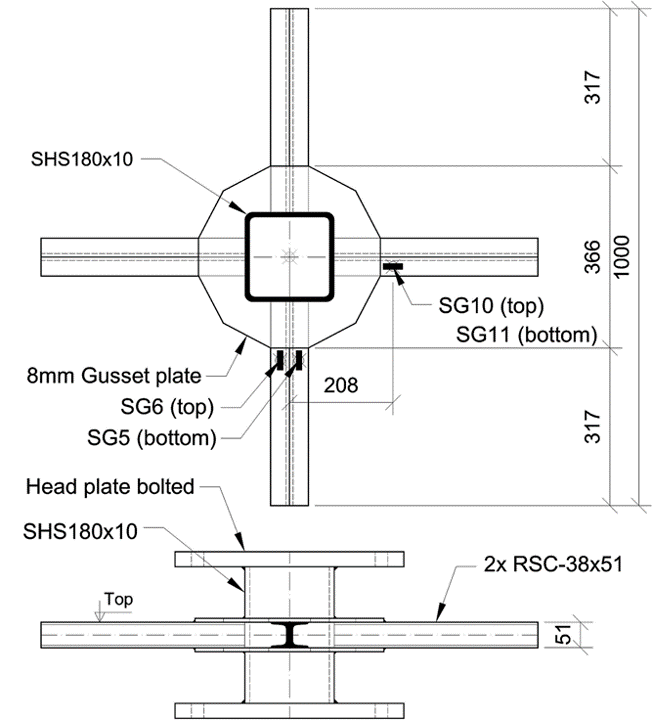
\includegraphics[width=\columnwidth]{Figures/e2010f9b.png}
    \caption{Shearhead detail studied in \cite{eder2010,EDER20111164}.}
    \label{e2010f9b}
    \end{figure}
\begin{figure}\centering
    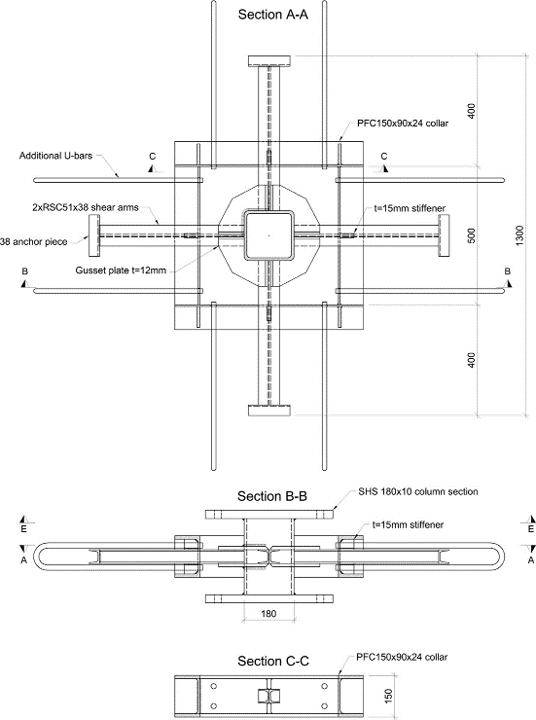
\includegraphics[width=\columnwidth]{Figures/e2012f2.png}
    \caption{Shearhead detail studied by \cite{EDER2012239}.}
    \label{e2012f2}
    \end{figure}
    \begin{figure}\centering
    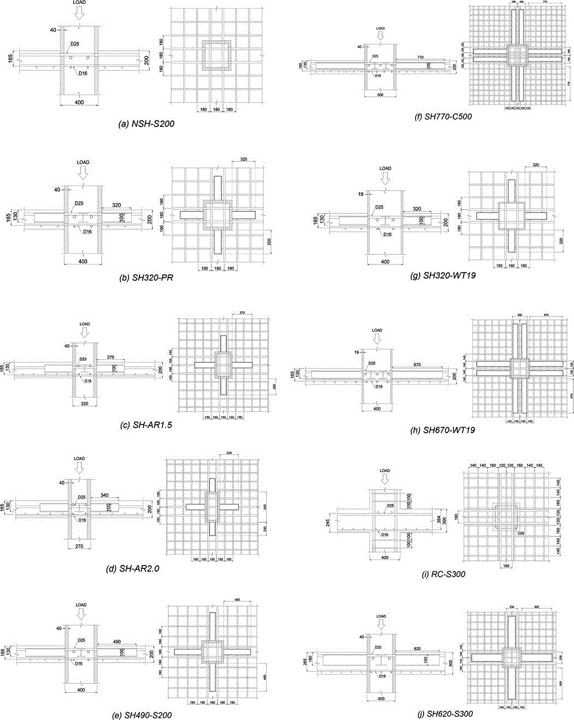
\includegraphics[width=\columnwidth]{Figures/k2014f2.png}
    \caption{\cite{kim2014shearhead} test specimens details.}
    \label{k2014f2}
    \end{figure}

    \begin{figure}\centering
    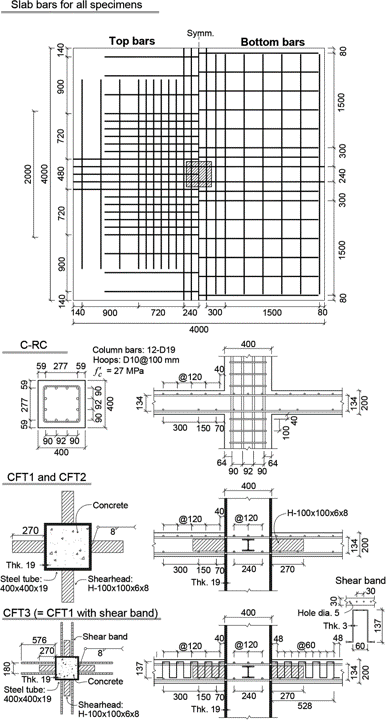
\includegraphics[width=\columnwidth]{Figures/l2019f3.png}
    \caption{\cite{lee2019seismic} specimen details.}
    \label{l2019f3}
    \end{figure}

    \begin{figure}\centering
    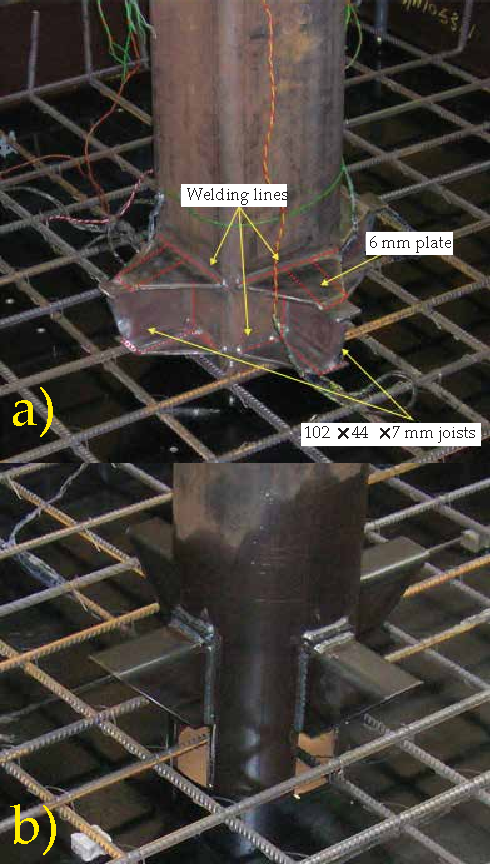
\includegraphics[width=\columnwidth]{Figures/y2014f2.pdf}
    \caption{Test specimens in \cite{yan2014}.}
    \label{l2014f2}
    \end{figure}
\begin{figure}\centering
    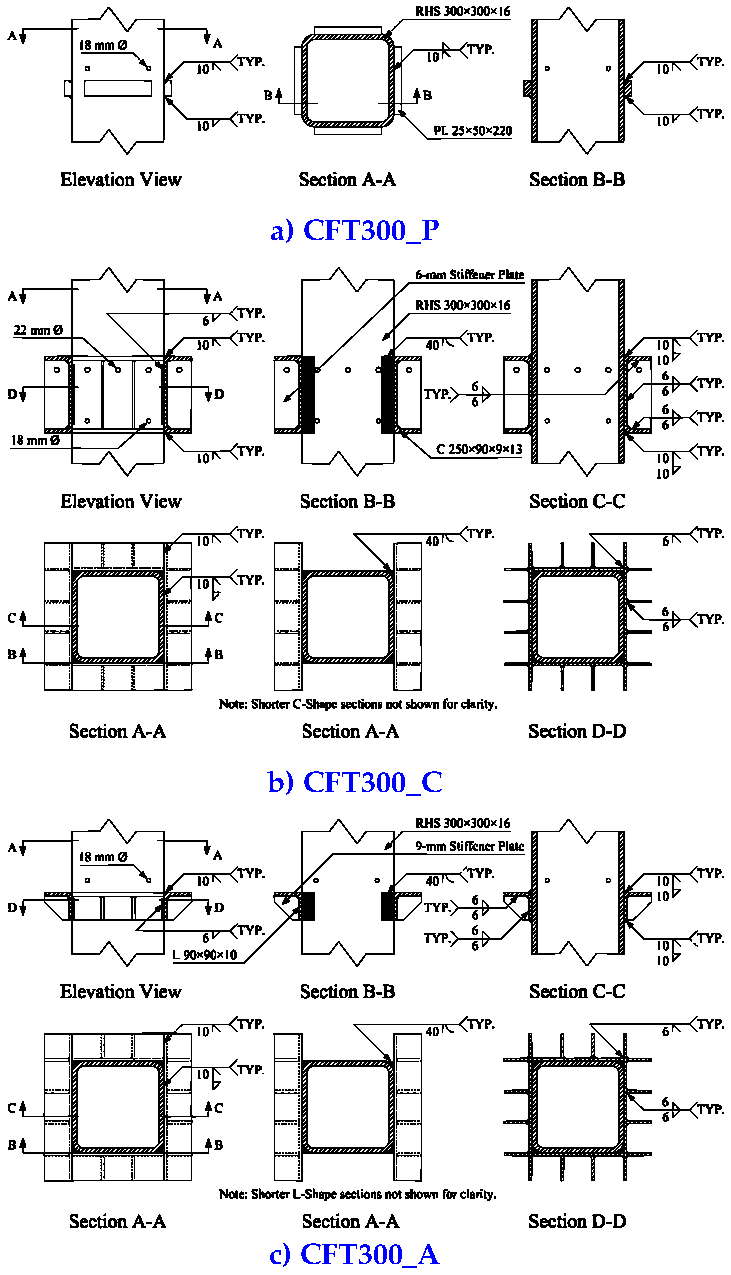
\includegraphics[width=\columnwidth]{Figures/tikzout/c2020f2.pdf}
    \caption{Shear enhancement detail\citep{chen2020}.}
    \label{c2020f2}
    \end{figure}
\begin{figure}\centering
    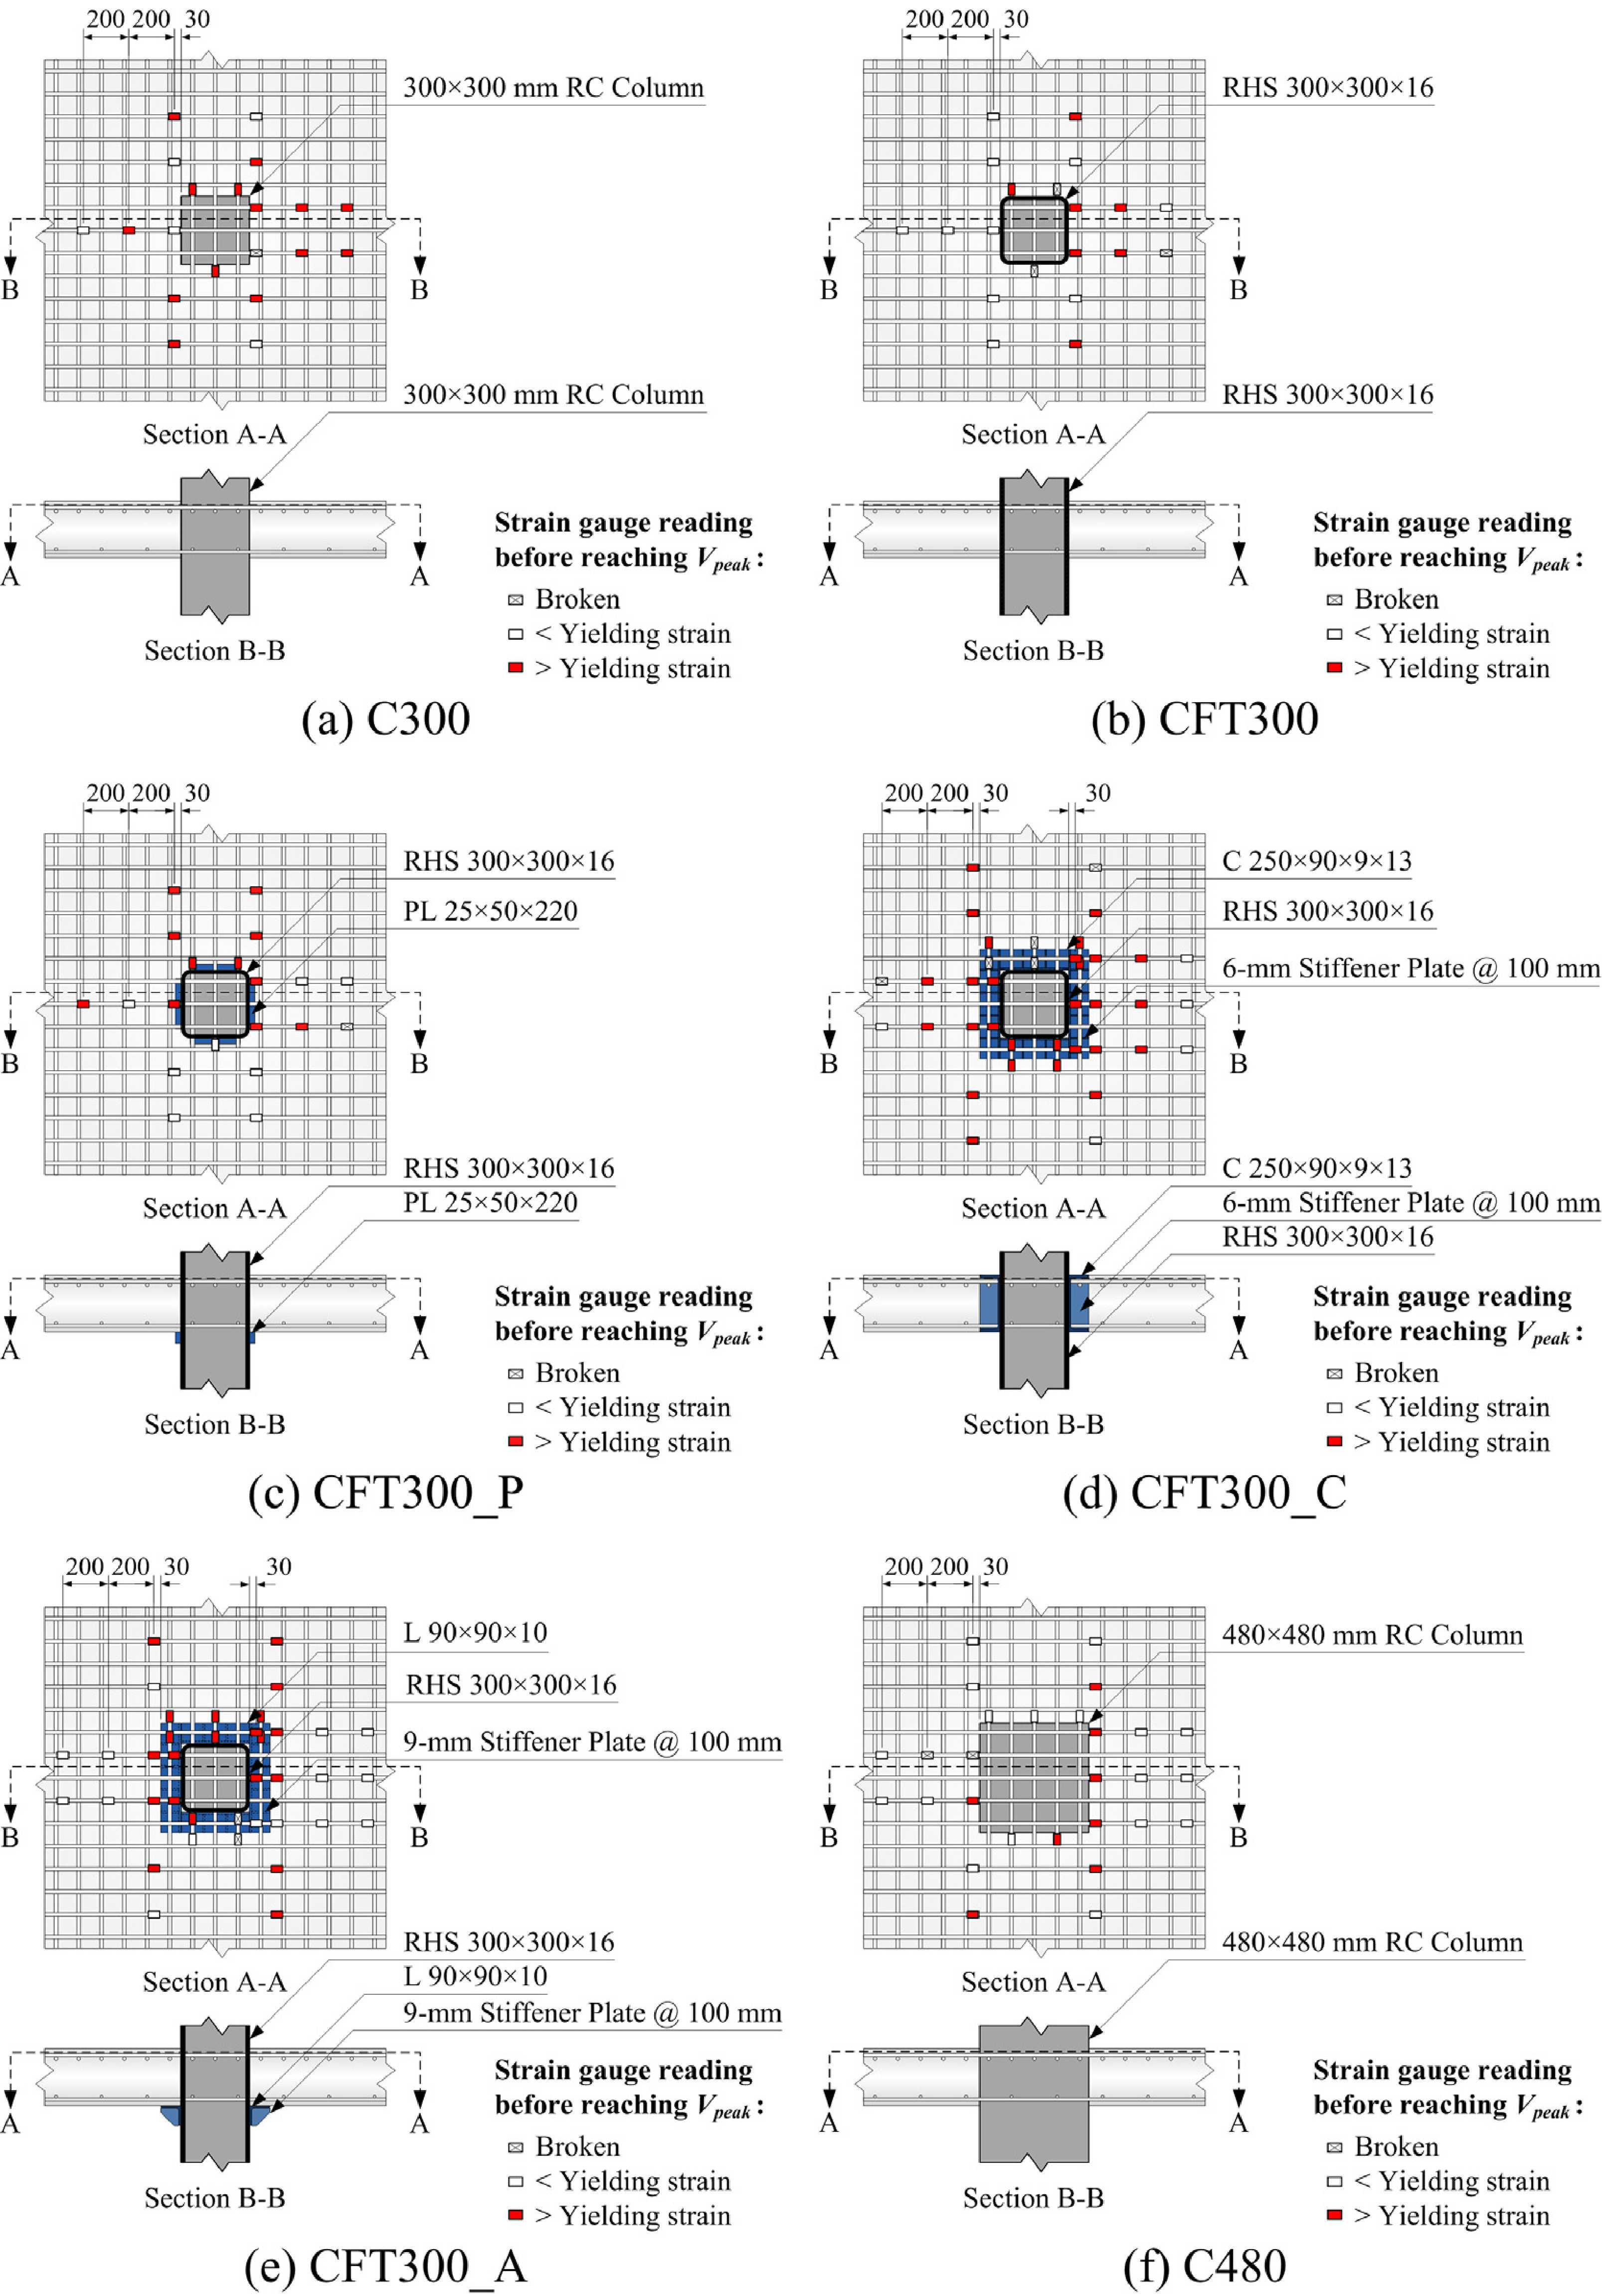
\includegraphics[width=\columnwidth]{Figures/c2020f3.pdf}
    \caption{Slab-column connection detail\citep{chen2020}.}
    \label{c2020f3}
    \end{figure}

The main disadvantage though lies in the discontinuity due to the smooth interface between the reinforced concrete slab and the steel or CFT column which is quite troubling when considering punching shear and punching shear resistance improvement alike what is practiced for concrete columns would not be applicable without mechanical means of connecting the steel column to the reinforced concrete flat slab.

This gave rise to research aimed at providing proper connection detail between the slab and CFT column to alleviate shear transfer most of which focused on using shearheads\citep{satoh2004experimental,lee2005,LEE2008418,yamaguchi2008experimental,eder2010,EDER20111164,EDER2012239,JU2013297,kim2014shearhead,yan2014,Bompa2016a,lee2019seismic,li2012,wang2013,yan2008} in the form of either I, T, rectangular steel tube or channel sections or shear studs welded on the column connection perimeter extending into the slab section\citep{yu2018}, while a combination of these was also reported \citep{LEE2008418}. 

\cite{satoh2004experimental} carried out three series of experimental studies on interior slab-column connections to evaluate lateral, punching shear and torsional behavior for a newly proposed connection(\ref{s2004f3}). \cite{LEE2008418} carried out full-scale tests on CFT column to RC flat plate connections subject to gravity loading aimed primarily at bettering connection detail and secondarily proposing a semi-analytical model of punching behavior for the proposed connections(\ref{l2008f2b}). Specimens with post-punching bars in \cite{LEE2008418} exhibited higher punching shear capacity and stiffness compared to those without that was attributed to better reinforcement of the concrete compression zone by these bars thus delaying concrete crushing while flexular anchoarge and shear key alterations had minor effects on punching shear capacity. In order to evaluate vertical load resistance capacity of a new CFT column-flat plate connection under various loading conditions \cite{yamaguchi2008experimental} tested three series of specimens fourty-six in total. 


In \cite{yan2014,lee2005,LEE2008418} top and bottom reinforcement were passed through the steel columns via provided holes which improves connection post-punching behavior and load bearing capacity. Following an experimental program \cite{chen2020} carried out six full-scaled tests of interior slab-column sub-assemblages under monotonically increased gravity loading with negligible eccentricity to study differences between reinforced concrete and CFT columns(\ref{c2020f3}) and also shear enhancement around the CFT column(\ref{c2020f2}). Test results showed that composite connections exhibited comparable punching shear strengths and failure modes while shear enhancement around the CFT column effectively shifted the failure plane away from the column faces hence increasing connection punching shear capacity\citep{chen2020}.

\cite{rafiee2021} conducted a reversed cyclic loading test on a half-scale post-tensioned (PT) flat slab-steel column specimen to examine the seismic details of their proposed exterior connection(\ref{r2021f2}).
\begin{figure}\centering
    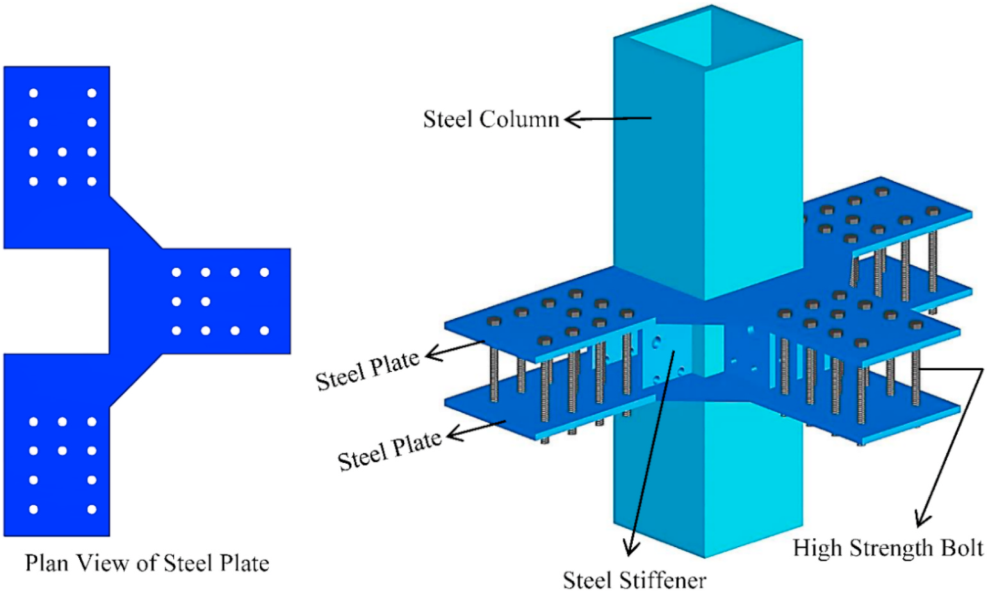
\includegraphics[width=\columnwidth]{Figures/r2021f2.png}
    \caption{Propose flat slab to steel column connection configuration\citep{rafiee2021}.}
    \label{r2021f2}
    \end{figure}
% Implementing nonlinear finite element analysis and critical shear crack theory \cite{setiawan2019} investigated internal slab-column connection behavior without shear reinforcement subject to seismic loading

\cite{yu2018} focused on developing a steel tubular column-flat slab connection following an experimental and numerical approach using shear studs welded around the column (\ref{yu2018f2}) as a simpler and more cost effective option compared to what had been proposed eariler by \cite{LEE2008418,yan2011,yan2014,yan2016} shown in \ref{yu2018f1}. 
\begin{figure}\centering
    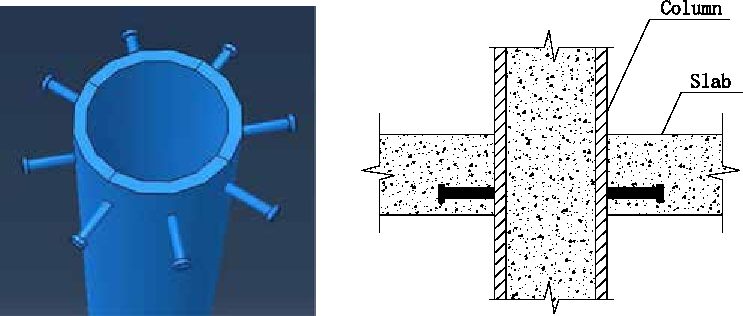
\includegraphics[width=\columnwidth]{Figures/yu2018f2.pdf}
    \caption{Shearhead configration proposed by \cite{yu2018}.}
    \label{yu2018f2}
    \end{figure}
\begin{figure}\centering
    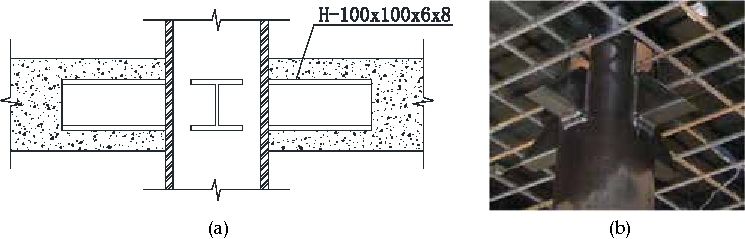
\includegraphics[width=\columnwidth]{Figures/yu2018f1.pdf}
    \caption{Shearhead configurations; a) Steel I shearhead sections welded on steel tubular column outer surface for reinforced concrete flat plate connection\citep{LEE2008418}; b) Shearhead inserted into steel tube column slots\citep{yan2016}.}
    \label{yu2018f1}
    \end{figure}
\cite{yan2016} ran an extensive parametric numerical study investigating punching shear resistance of hybrid steel tubular column to reinforced concrete flat slab connection using shearhead arms in which study parameters included column shape, shearhead arm properties and slab reinforcement. \citep{yu2020} in a  subsequent numerical and analytic investigation proposed an innovative shear connection for flat slab to steel column connections using welded shear studs, steel plates and bent-up bars(\ref{y2020f3}) that evolved out of \cite{yu2018}. 
\begin{figure}\centering
    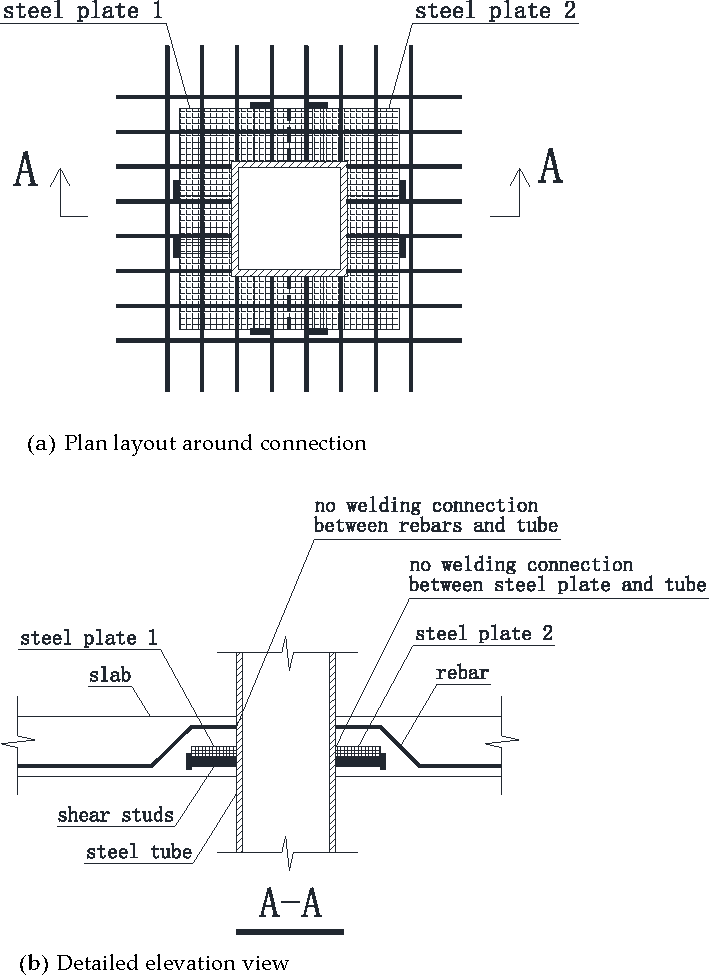
\includegraphics[width=\columnwidth]{Figures/y2020f3.pdf}
    \caption{Proposed steel tube to concrete flat slab connection detail\citep{yu2020}.}
    \label{y2020f3}
    \end{figure}
\cite{zhang2018} proposed a new connection mechanism between prefabricated reinforced concrete flat slab and square steel tube column(\ref{z2018f1}) through an experimental test followed by a complementary numerical simulation. The connection inhibits plastic deformations in the cantilever beams which are replaceable after an earthquake\citep{zhang2022}.
\begin{figure*}\centering
    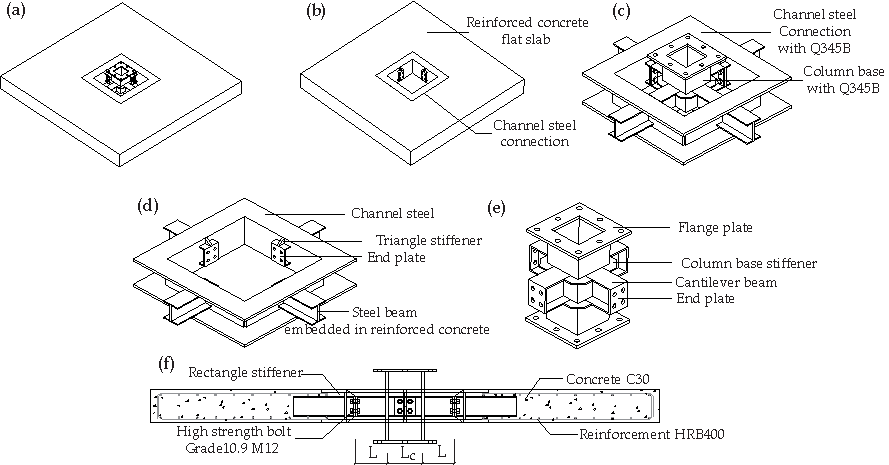
\includegraphics[width=\textwidth]{Figures/z2018f1.pdf}
    \caption{Configuration of prefabricated reinforced concrete flat slab to square steel tube column connection\citep{zhang2018}: a) Slab-column connection; b) Reinforced concrete flat slab and channel steel section; c) Column base connection; d) Channel steel connection; e) Column base; f) Connection cross-section.}
    \label{z2018f1}
    \end{figure*}
A total of nine simply supported slab-column connection specimens were subjected to vertical load by \cite{zhou2021} in addition to a finite element study to investigate punching shear behavior of slab-column connections embedded with steel skeletons which changed the mode of failure from punching shear into flexural punching(\ref{z2021f3}).
\begin{figure*}\centering
    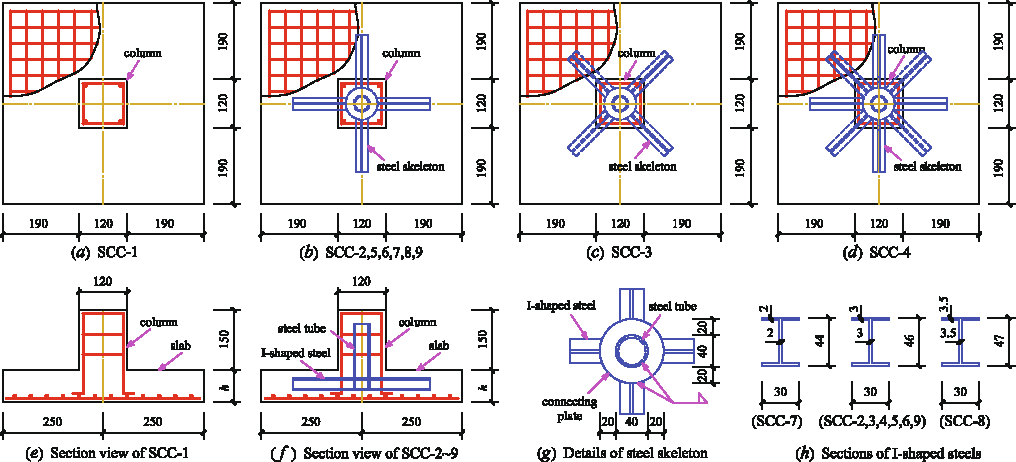
\includegraphics[width=\textwidth]{Figures/z2021f3.pdf}
    \caption{Specimen details\citep{zhou2021}.}
    \label{z2021f3}
    \end{figure*}
Punching shear performance of edge steel column to flat slab connection via a modified shearhead assembly was investigated by \cite{ngekpe2019} through experimental testing and numerical simulations that ended in punching shear governed by shear regardless of shearhead connection robustness. \cite{zhang2022} investigated seismic behavior of a prefabricated reinforced concrete flat slab to steel tubular column connection through `I' shaped cantilevered beams introduced so as to enhance ductility and energy dissipation. \cite{luu2022} proposed innovative slab to CFT column conections for unbonded post-tensionned concrete slabs through an experimental investigation conducting six large-scale tests(\ref{l2022f2}).
\begin{figure*}\centering
    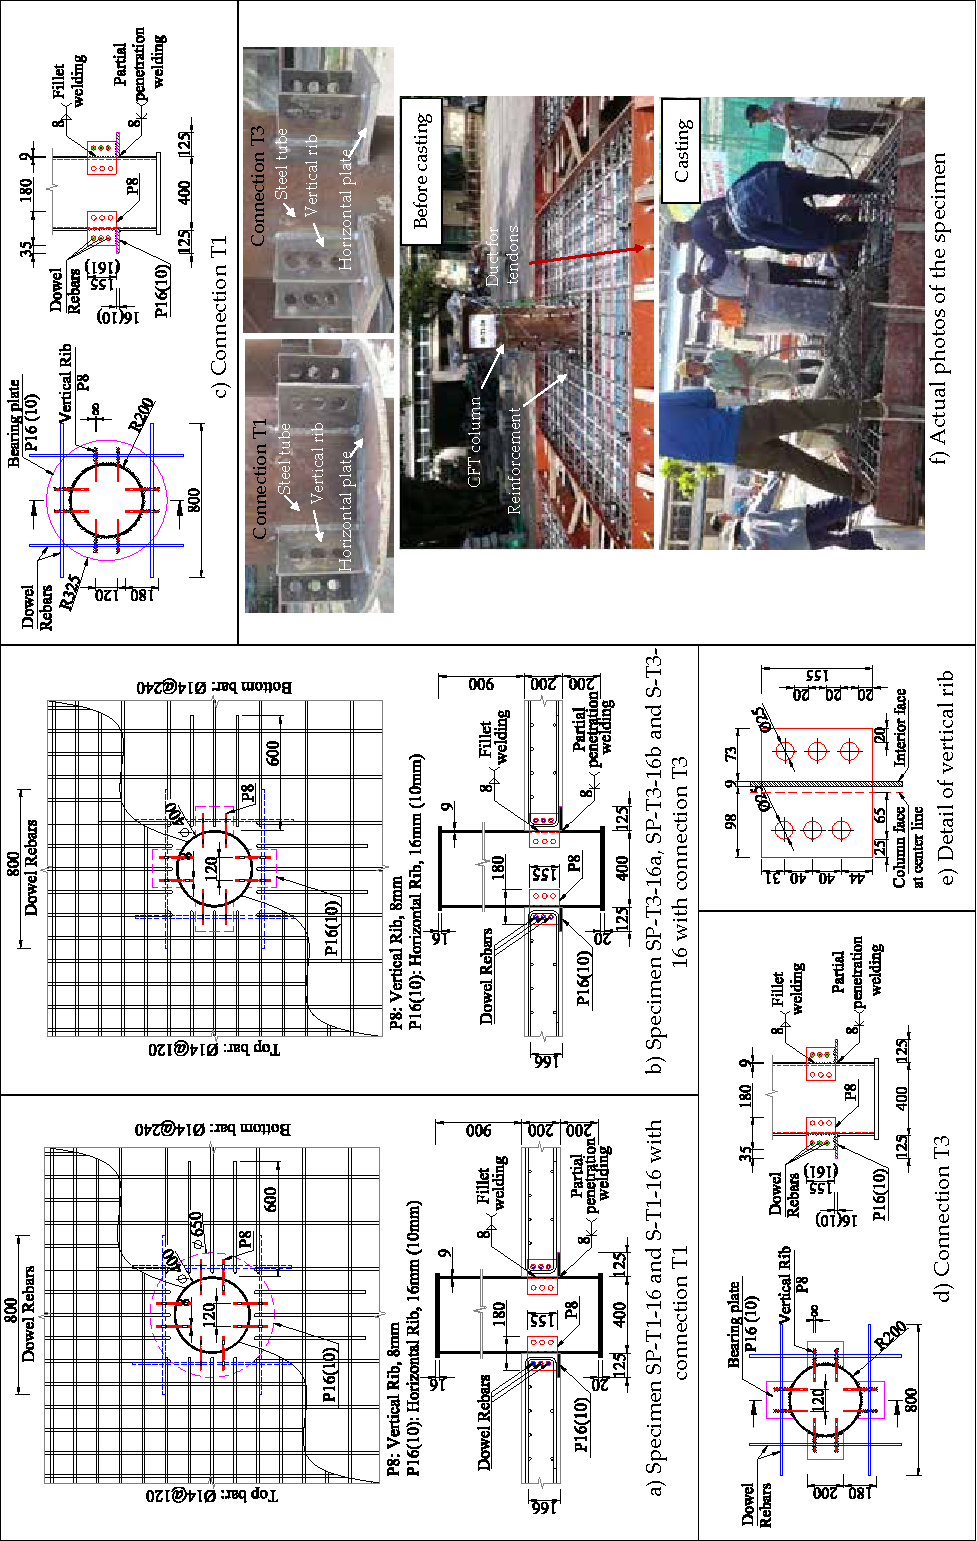
\includegraphics[height=\textwidth,angle=-90]{Figures/l2022f2.pdf}
    \caption{Flat slab-CFT column connection joint designs\citep{luu2022}.}
    \label{l2022f2}
    \end{figure*}
\cite{chen2023} implemented steel plates as batten plates, confined plates and drop plates for a slab-column connection with a spatial steel drop panel in an experimental investigation varying drop plate size, batten plate length and whether drop plates have slits for five specimens under monotonically increasing gravity load to ascertain connection detail effects on the punching shear performance(\ref{c2023f2}).
\begin{figure}\centering
    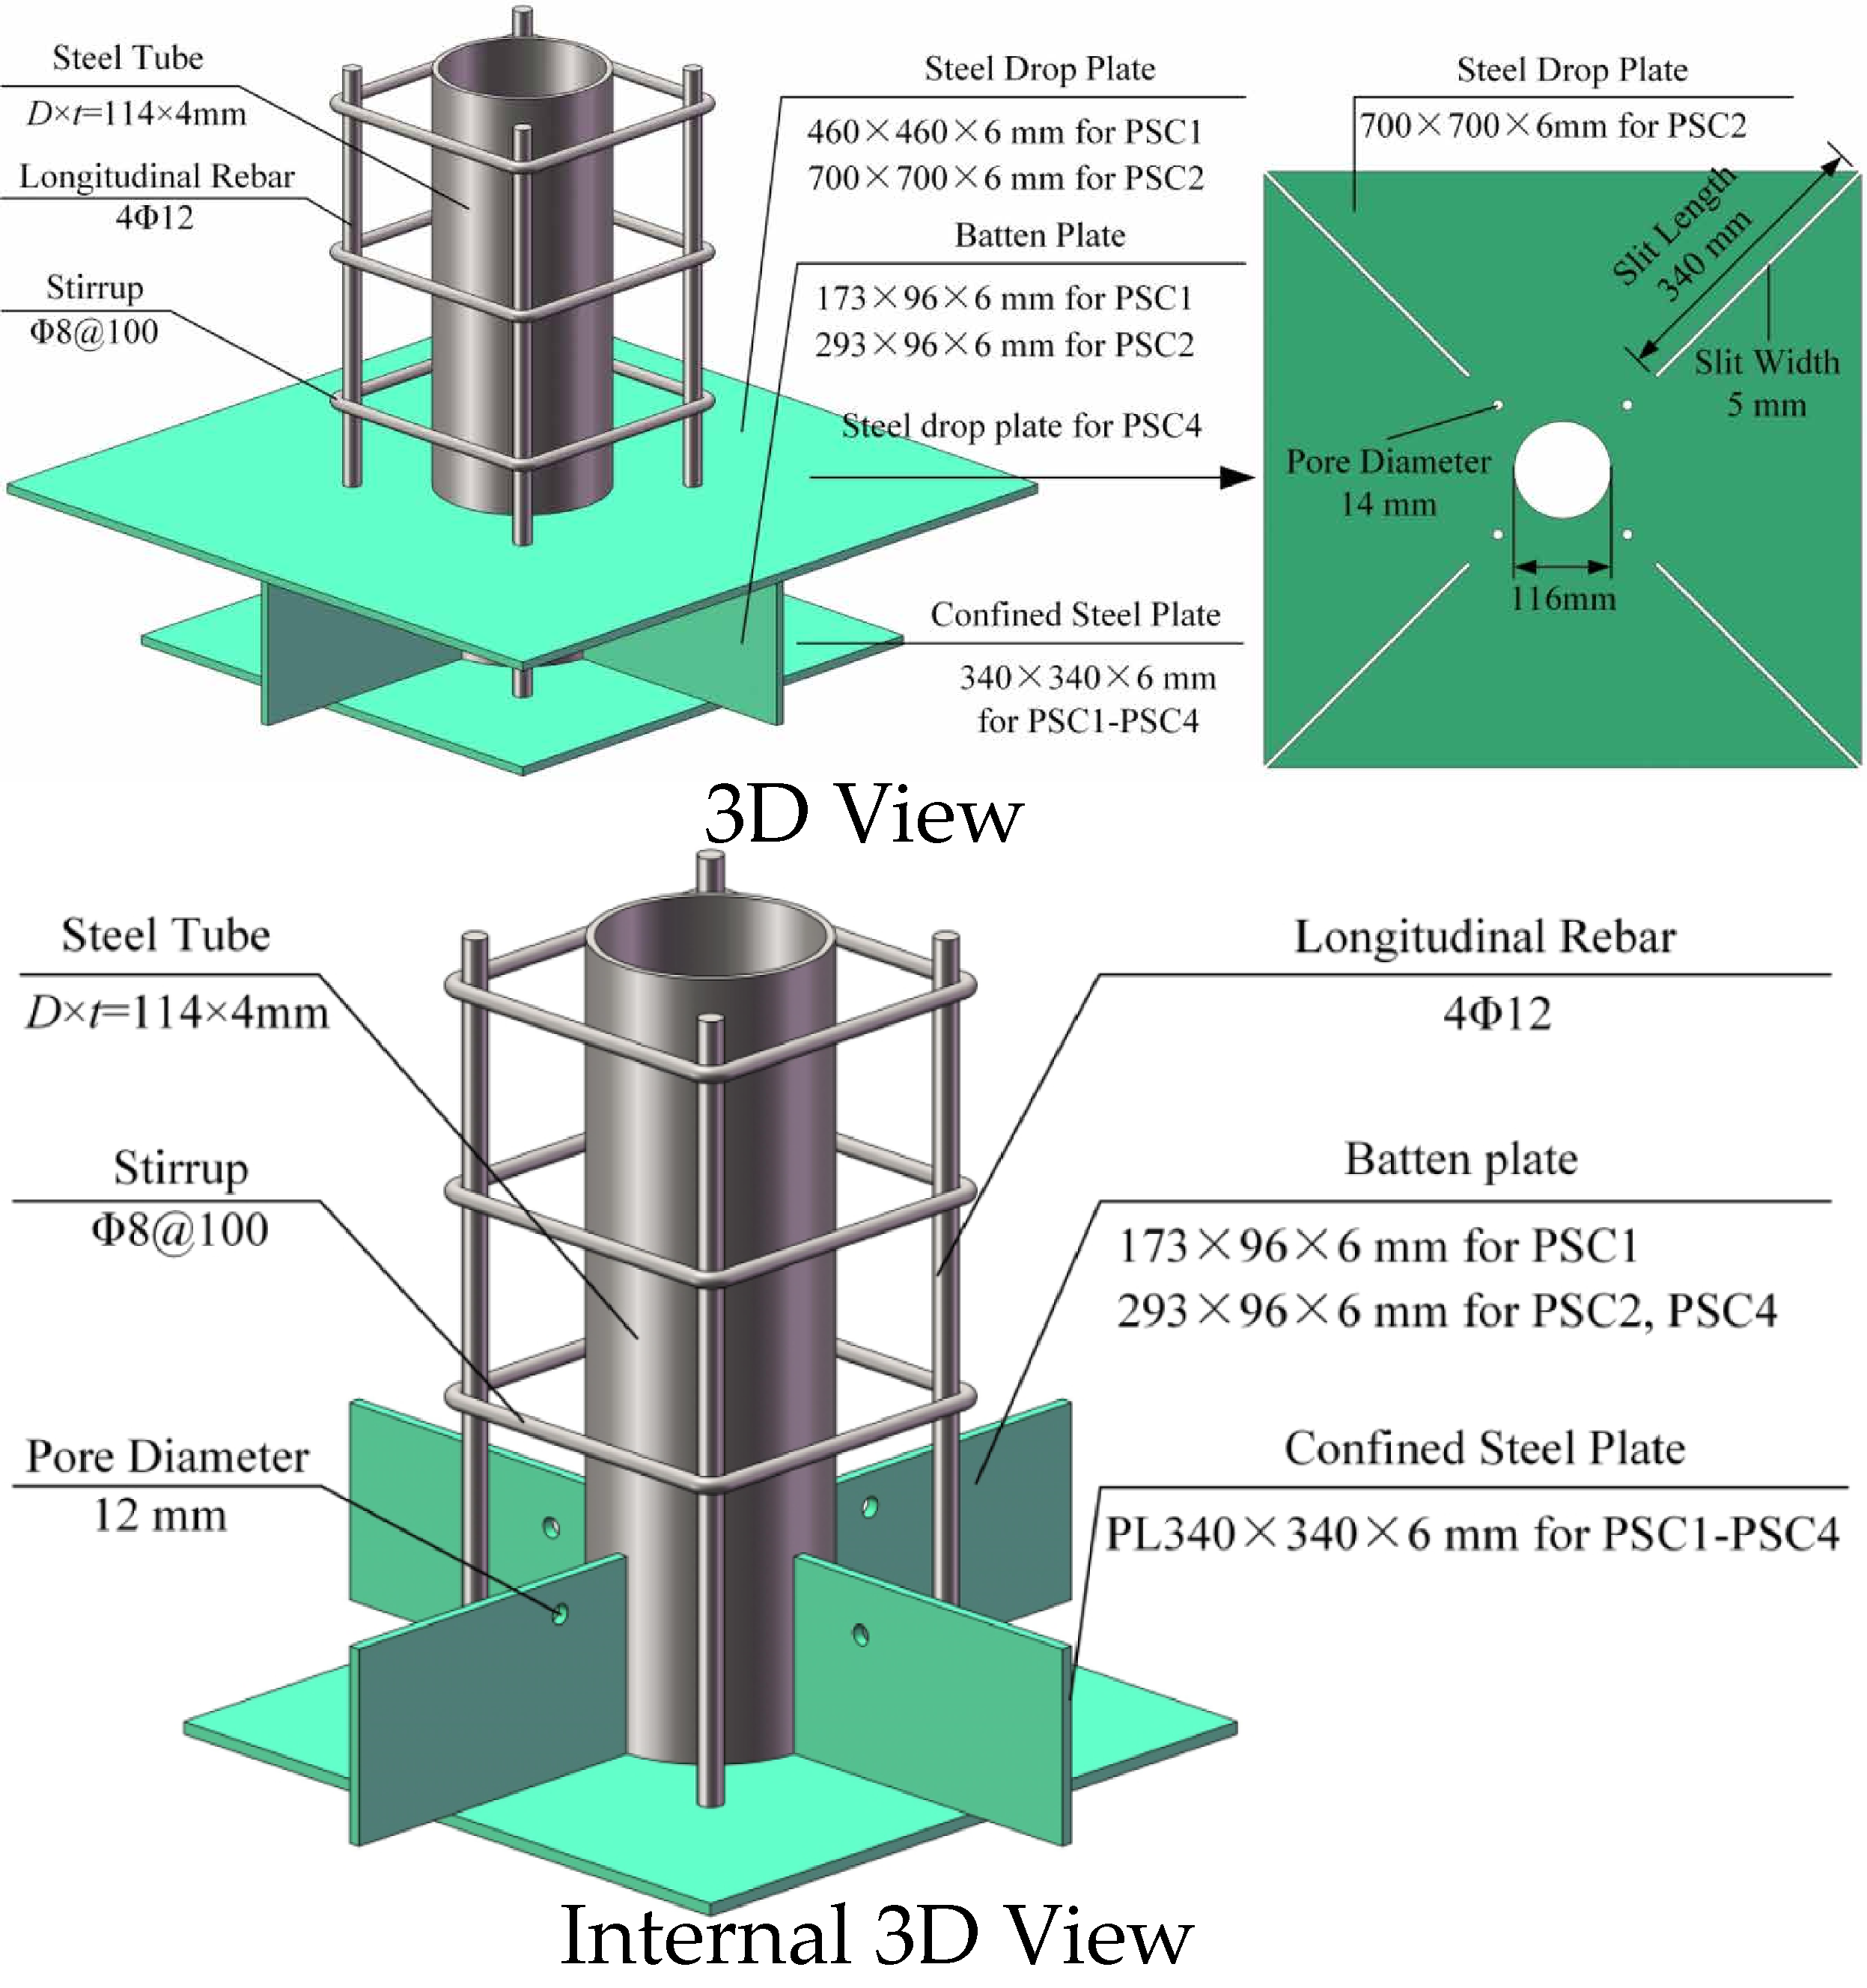
\includegraphics[height=\columnwidth]{Figures/c2023f2.pdf}
    \caption{Spatial steel drop panel details for specimens PSC1, PSC2 and PSC4 \citep{chen2023}.}
    \label{c2023f2}
    \end{figure} 